\section{去毛刺}
相关命令:\nameref{cmd:rglitches}

地震仪器偶尔会出现问题,导致连续地震数据流中出现尖锋或者数据丢失。
这些所谓的毛刺,肉眼很容易识别,但是在使用程序自动处理数据时却很
容易被误认为是地震信号,因而需要在数据分析之前将毛刺去除。
\texttt{rglitches} 命令可以在某种程度上检测并去除地震信号中的毛刺。
毛刺在模拟地震记录中很常见,现在的数字地震记录中则很少见到,因而实
际上很少需要执行这一步操作。

\texttt{rglitches} 的效果可以从图 \ref{fig:deglitches} 中直观地看到。
\begin{figure}[H]
\centering
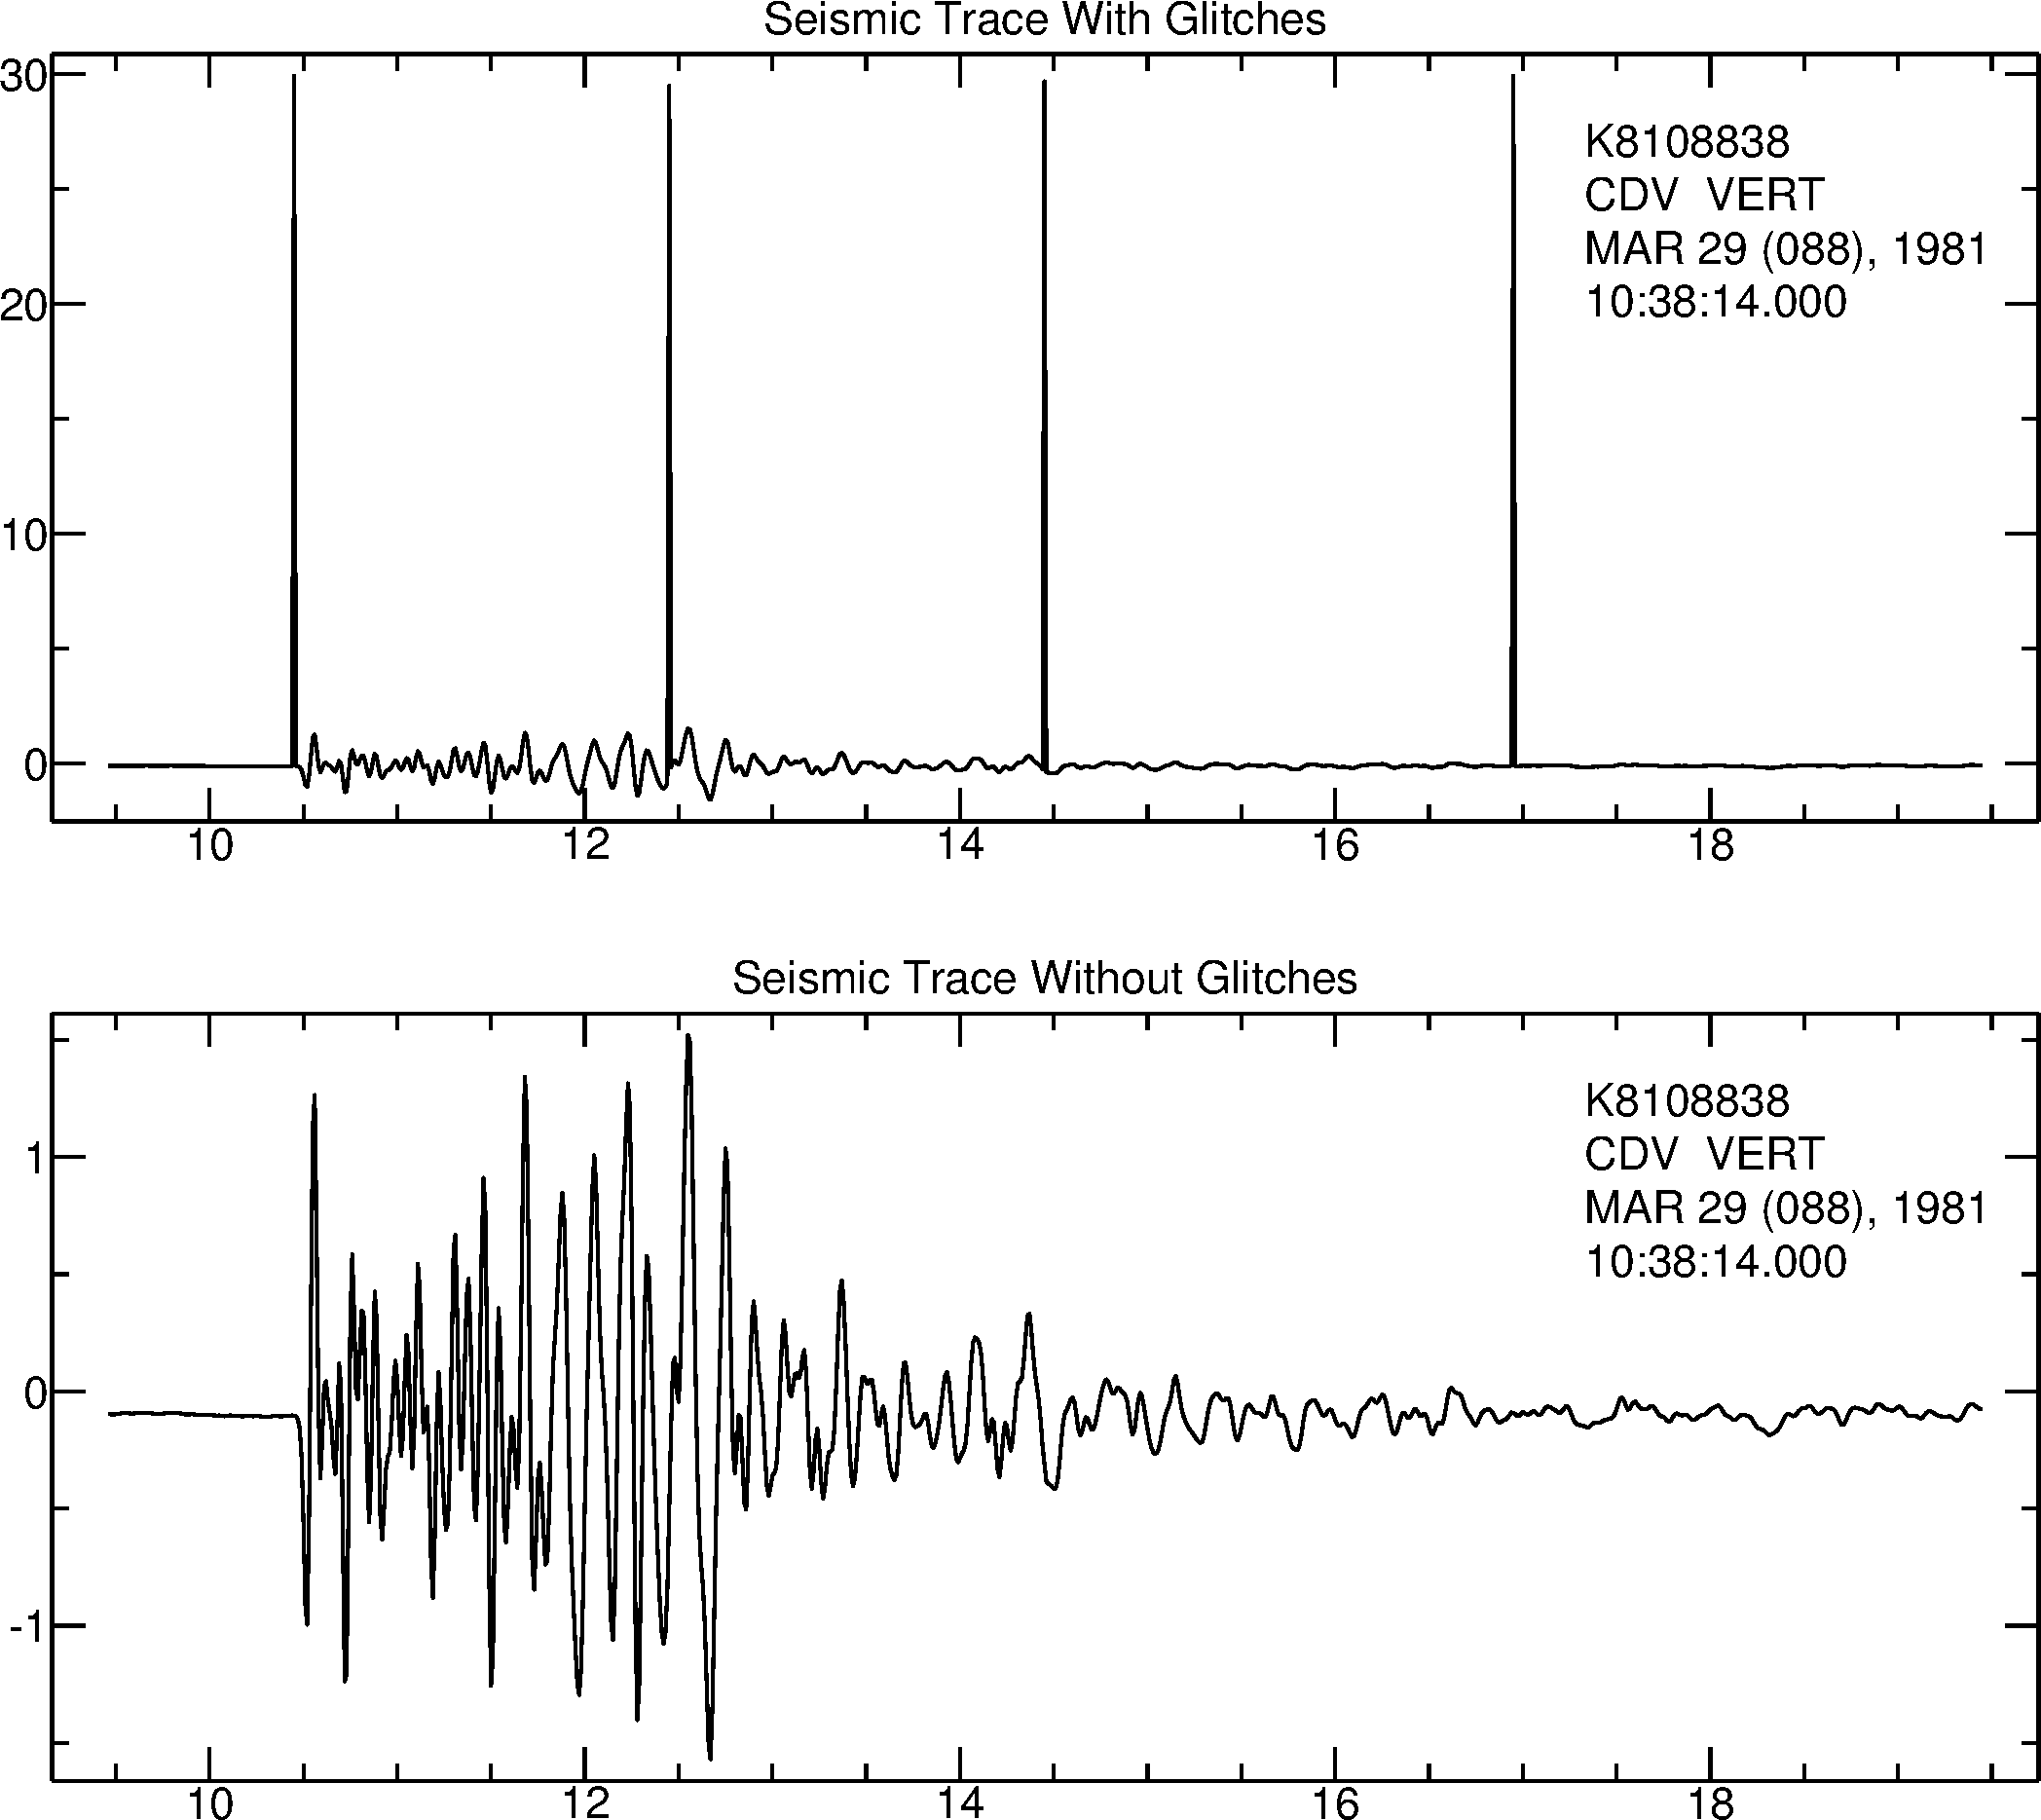
\includegraphics[width=0.95\textwidth]{rglitches}
\caption[地震波形去毛刺]{地震波形去毛刺。上图为包含glitches的地震信号,
    下图为去除glitches后的地震信号。}
\label{fig:deglitches}
\end{figure}
